% !TeX root = ../tesi.tex
% !TeX encoding = UTF-8
% !TeX spellcheck = it_IT

\chapter{Localizzazione delle aree modificate e descrizione}
\label{chap:localizzazione-descrizione}

In questo capitolo descrivo come ricavo le regioni sospette dalle immagini selezionate e ne rappresento il contenuto mediante testo. Presento TruFor come componente esterno della pipeline (Sezione~\ref{sec:materiali-trufor}), poi il test preliminare su 100 immagini annotate (Sezione~\ref{sec:metodi-trufor-benchmark}) e l'applicazione al dataset filtrato (Sezione~\ref{sec:metodi-trufor-esecuzione}). Illustro quindi la creazione delle maschere e la loro valutazione (Sezione~\ref{sec:metodi-maschere}). Concludo con la descrizione tramite BLIP e OCR, i risultati ottenuti e gli esempi visivi (Sezione~\ref{sec:metodi-descrizioni}).

\section{TruFor come componente esterno}
\label{sec:materiali-trufor}

Utilizzo TruFor, descritto nel Capitolo~\ref{chap:background} e nel paper~\cite{Guillaro_2023_CVPR}. Clono il \href{https://github.com/grip-unina/TruFor}{repository ufficiale} nella cartella \path{TruFor/} del progetto. Mantengo separati il codice di TruFor e gli script delle elaborazioni successive. Uso il framework come componente a scatola nera: fornisco gli input e acquisisco gli output del modello. Mantengo i pesi preaddestrati durante tutte le elaborazioni.

Lo script \path{scripts/trufor.py} richiama \path{TruFor/TruFor_train_test/test.py}. La configurazione selezionata è \texttt{trufor\_ph3}; il file dei pesi è \path{TruFor/TruFor_train_test/weights/trufor_ph3/best.pth.tar}. Centralizzo i percorsi e i parametri di esecuzione in \path{scripts/config.py}.

La copia locale include modifiche per adattare l’esecuzione alle risorse del dispositivo: un limite massimo di pixel in ingresso e ottimizzazioni per il supporto della GPU. Descrivo il ridimensionamento dell'input nella Sezione~\ref{sec:metodi-trufor-esecuzione}. Questi interventi riguardano l'esecuzione del modello preaddestrato. 

Per aggiornare TruFor basta sostituire la cartella \path{TruFor/} con la nuova versione, riapplicare gli adattamenti per il dispositivo e adeguare gli script della pipeline alle eventuali variazioni dell’interfaccia e degli output.

\subsection{Organizzazione degli input e degli output}
\label{subsec:materiali-trufor-output}

Uso \path{scripts/temp/} come cartella di lavoro. Al suo interno, \path{images/} contiene i collegamenti ai file selezionati come input (Sottosezione~\ref{subsec:dataset-campione-filtrato}) e \path{npz/} contiene gli archivi prodotti da TruFor. Conservo i punteggi associati ai post in \path{dataset_filtered.csv}.

Per ogni file elaborato acquisisco un archivio NumPy, con estensione \texttt{.npz}. Il nome conserva quello dell'input e aggiunge l'estensione, per esempio \path{picture.jpg.npz}. Riporto nella Tabella~\ref{tab:materiali-trufor-output} i campi utilizzati dal progetto. Per il significato delle due mappe richiamo la Sottosezione~\ref{subsec:background-trufor-architettura}.

\begin{table}[htbp]
    \centering
    \small
    \caption{Campi degli output di TruFor utilizzati nella pipeline~\cite{Guillaro_2023_CVPR}.}
    \label{tab:materiali-trufor-output}
    \begin{tabular}{@{}lp{0.75\linewidth}@{}}
        \toprule
        Campo & Contenuto e utilizzo \\
        \midrule
        \texttt{map} & Mappa delle anomalie, usata per individuare le regioni sospette. \\
        \addlinespace
        \texttt{conf} & Mappa di confidenza, usata nell'elaborazione delle previsioni per pixel. \\
        \addlinespace
        \texttt{score} & Punteggio globale, riportato nella tabella del dataset come \texttt{trufor\_score}. \\
        \addlinespace
        \texttt{imgsize} & Altezza e larghezza originali, in pixel. \\
        \bottomrule
    \end{tabular}
\end{table}

Indico con $t_i$ il punteggio globale prodotto per l'immagine $i$ (Sottosezione~\ref{subsec:background-trufor-output}).

\section{Test preliminare di TruFor sul dataset}
\label{sec:metodi-trufor-benchmark}

\subsection{Annotazione manuale del campione}
\label{subsec:materiali-trufor-annotazioni}

Prima dell'elaborazione completa considero un sottoinsieme eterogeneo di 100 contenuti del dataset, scelti casualmente tra i post contenenti immagini. Assegno manualmente a ciascuno un'etichetta globale, che indico con $z_i$: 0 per i media che giudico autentici e 1 per quelli che credo alterati. Il campione comprende 38 casi nella prima classe e 62 nella seconda. Uso queste annotazioni come ground truth del confronto. Seguendo la convenzione definita nella Sottosezione~\ref{subsec:background-rilevamento-localizzazione}, considero positiva la classe ``alterato``, indipendentemente dal tipo di alterazione.

Registro le etichette in \path{scripts/temp/trufor_truth.csv}, con i campi \texttt{filename} e \texttt{label}. Il primo identifica il file senza estensione; il secondo contiene $z_i$.

Attribuisco alla verifica un carattere esplorativo. Le annotazioni riflettono il mio giudizio come unico annotatore e servono a esaminare il comportamento di TruFor sulla raccolta. Le etichette globali permettono di valutare il rilevamento; la valutazione della localizzazione richiede invece un riferimento per ciascun pixel.

\subsection{Protocollo di valutazione}
\label{subsec:trufor-test-protocollo}

Eseguo TruFor sul campione descritto nella Sottosezione~\ref{subsec:materiali-trufor-annotazioni}. Confronto la previsione del modello con il mio giudizio sull'autenticità di ciascun contenuto.

Per ricavare una decisione dal punteggio $t_i$, applico la soglia $\tau=0{,}25$, impostata tramite \texttt{TRUFOR\_THRESHOLD}. Indico con $\widehat{z}_i$ la classe prevista:
\begin{equation}
    \widehat{z}_i =
    \begin{cases}
        1 & \text{se } t_i > \tau, \\
        0 & \text{se } t_i \leq \tau.
    \end{cases}
    \label{eq:metodi-trufor-soglia}
\end{equation}
Uso questa soglia soltanto per la verifica del rilevamento. L'elaborazione delle mappe usa parametri distinti.

Calcolo la matrice di confusione tra $z_i$ e $\widehat{z}_i$, insieme ad accuratezza, precisione, richiamo e F1-score. Confronto l'accuratezza con quella ottenuta assegnando sempre la classe più frequente nel campione. Calcolo anche l’AUC (Area Under the Curve) direttamente dai punteggi, per valutare la capacità di distinguere i casi autentici da quelli alterati senza fissare un’unica soglia decisionale.

Affianco alla configurazione scelta un confronto delle soglie da $0{,}20$ a $0{,}50$, con passo $0{,}05$. Per ciascuna ricalcolo le metriche sullo stesso campione. Uso queste prove per un benchmark preliminare della soglia decisionale e interpreto le misure come risultati esplorativi sui casi annotati. Mantengo fissi i pesi del modello.

Salvo il confronto in \path{trufor_confusion_matrix.txt}. Il documento contiene anche gli identificatori dei falsi positivi e dei falsi negativi, con i rispettivi punteggi, per consentire l'ispezione dei singoli casi.

\subsection{Risultati del test e confronto delle soglie}
\label{subsec:trufor-test-risultati}

Riporto nella Tabella~\ref{tab:trufor-confusione} il confronto con le annotazioni manuali.

\begin{table}[htbp]
    \centering
    \small
    \caption{Matrice di confusione sui 100 casi annotati, con soglia $0{,}25$. Le righe indicano le mie annotazioni; le colonne indicano le previsioni di TruFor.}
    \label{tab:trufor-confusione}
    \begin{tabular}{@{}lrrr@{}}
        \toprule
        Annotazione manuale & Previsto autentico & Previsto alterato & Totale \\
        \midrule
        Autentico & 24 & 14 & 38 \\
        Alterato & 11 & 51 & 62 \\
        \midrule
        Totale & 35 & 65 & 100 \\
        \bottomrule
    \end{tabular}
\end{table}

La Tabella~\ref{tab:trufor-confronto-soglie} mostra il confronto tra le soglie. Tra i valori esaminati, $0{,}25$ produce l'accuratezza e l'F1-score maggiori. La soglia $0{,}20$ favorisce il richiamo, mentre $0{,}50$ produce la precisione maggiore.

\begin{table}[htbp]
    \centering
    \small
    \caption{Confronto delle soglie sullo stesso campione di 100 casi. Il grassetto evidenzia la configurazione usata nel benchmark.}
    \label{tab:trufor-confronto-soglie}
    \begin{tabular}{@{}rrrrr@{}}
        \toprule
        Soglia & Accuratezza & Precisione & Richiamo & F1-score \\
        \midrule
        $0{,}20$ & $72{,}00\%$ & $72{,}97\%$ & $87{,}10\%$ & $0{,}7941$ \\
        $\mathbf{0{,}25}$ & $\mathbf{75{,}00\%}$ & $\mathbf{78{,}46\%}$ & $\mathbf{82{,}26\%}$ & $\mathbf{0{,}8031}$ \\
        $0{,}30$ & $73{,}00\%$ & $79{,}66\%$ & $75{,}81\%$ & $0{,}7769$ \\
        $0{,}35$ & $70{,}00\%$ & $79{,}63\%$ & $69{,}35\%$ & $0{,}7414$ \\
        $0{,}40$ & $67{,}00\%$ & $80{,}85\%$ & $61{,}29\%$ & $0{,}6972$ \\
        $0{,}45$ & $62{,}00\%$ & $81{,}58\%$ & $50{,}00\%$ & $0{,}6200$ \\
        $0{,}50$ & $61{,}00\%$ & $82{,}86\%$ & $46{,}77\%$ & $0{,}5979$ \\
        \bottomrule
    \end{tabular}

    \medskip
    \begin{minipage}{0.9\linewidth}
        \small
        L'accuratezza del riferimento che assegna sempre la classe maggioritaria, ``alterato'', è pari al $62{,}00\%$. L'AUC è pari a $0{,}7538$ ed è calcolata dai punteggi continui, indipendentemente dalla soglia scelta.
    \end{minipage}
\end{table}

\section{Applicazione di TruFor al dataset filtrato}
\label{sec:metodi-trufor-esecuzione}

Dopo la verifica preliminare applico TruFor all'intero dataset filtrato. Lo script \path{scripts/trufor.py} avvia il programma di inferenza in un processo separato, usando l'interprete Python dell'ambiente corrente. Fornisco come argomenti le cartelle degli input e degli output e il limite di risoluzione.

Imposto \texttt{TRUFOR\_MAX\_PIXELS} a 6.000.000. Se un input supera il limite il caricatore lo ridimensiona mantenendo le proporzioni. Il modello esegue l'inferenza sul contenuto; il programma riporta poi le mappe alle dimensioni originali tramite interpolazione bilineare. Il punteggio globale deriva dall'input effettivamente elaborato.

Organizzo l'esecuzione in gruppi di 50 file e inserisco una pausa di 180 secondi tra gruppi consecutivi. Per ogni gruppo lo script prepara una cartella temporanea con i collegamenti agli originali da elaborare e avvia un nuovo processo. Il programma carica il modello una volta per gruppo ed elabora un file alla volta. Questa organizzazione regola il carico della macchina durante l'esecuzione.

Gli output vengono salvati in \path{scripts/temp/npz/}, un file \texttt{.npz} dopo ogni elaborazione completata. Se un gruppo si interrompe per un crash, restano disponibili i risultati dei gruppi precedenti e quelli già salvati del gruppo interrotto.

Per esecuzioni successive il programma salta gli input associati a output già presenti; posso quindi riprendere il lavoro dagli elementi mancanti. Il riuso degli output presuppone la stessa configurazione di elaborazione; un cambio di configurazione richiede di rigenerarli o salvarli in una cartella distinta.

Estraggo dagli archivi il campo \texttt{score}, descritto nella Tabella~\ref{tab:materiali-trufor-output}, e lo rinomino \texttt{trufor\_score}. Aggiorno la tabella \path{dataset_filtered.csv} tramite \texttt{filename}, ottenuto dal nome dell'output senza le estensioni. L'unione conserva solo le osservazioni con una corrispondenza. Mantengo le mappe negli archivi per i passaggi successivi della pipeline.

\section{Creazione e valutazione delle maschere}
\label{sec:metodi-maschere}

Uso \path{scripts/mask.py} per selezionare le regioni sospette da fornire alla successiva descrizione testuale. Uso le mappe di anomalia e confidenza salvate da TruFor nei file .npz, descritti nella Sottosezione~\ref{subsec:materiali-trufor-output}. Applico questo passaggio a tutte le immagini con output disponibile, indipendentemente dalla decisione sul punteggio globale $t_i$.

\subsection{Annotazioni delle regioni e maschere di riferimento}
\label{subsec:materiali-maschere-riferimento}

Per valutare la localizzazione delle maschere uso le stesse 100 immagini della Sottosezione~\ref{subsec:materiali-trufor-annotazioni}. Disegno manualmente una maschera per ciascuna immagine: coloro di bianco le regioni che credo alterate e di nero quelle autentiche. Conservo queste maschere di riferimento in \path{masked_truth/}, associandole agli originali tramite il nome del file.

Svolgo le due valutazioni in modo indipendente. L'etichetta $z_i$, definita nella Sottosezione~\ref{subsec:materiali-trufor-annotazioni}, esprime il mio parere sull'aspetto complessivo dell'immagine. La maschera registra il giudizio sulle singole regioni. Un contenuto classificato globalmente come autentico può quindi avere regioni annotate come alterate, anche per un totale di aree maggiore della metà della superficie. L'etichetta globale non deriva dalla percentuale di pixel bianchi.

La maschera binaria indica quali pixel conservare e quali escludere, secondo la segmentazione descritta nella Sottosezione~\ref{subsec:background-rilevamento-localizzazione}. Applicandola all'originale ottengo l'immagine mascherata, che mantiene i colori dei pixel selezionati e rende neri quelli esclusi.

Per misurare la sovrapposizione uso l'\emph{Intersection over Union} (IoU). Indico con $P_i$ l'insieme dei pixel previsti come alterati e con $T_i$ quello dei pixel alterati nel riferimento manuale:
\begin{equation}
    \operatorname{IoU}_i=\frac{|P_i\cap T_i|}{|P_i\cup T_i|}.
    \label{eq:maschere-iou}
\end{equation}
La misura vale 1 quando le regioni coincidono e 0 quando sono disgiunte. Se entrambi gli insiemi sono vuoti, adotto la convenzione $\operatorname{IoU}_i=1$. Calcolo la IoU sia aggregando le intersezioni e le unioni di tutte le immagini, sia facendo la media dei valori ottenuti per ciascuna immagine. Nel primo caso incidono maggiormente le immagini con regioni di unione più estese; nel secondo ogni immagine ha lo stesso peso.

\subsection{Dalle mappe all'immagine mascherata}
\label{subsec:metodi-maschere-creazione}

Uso le mappe di anomalia e confidenza già riportate alle dimensioni originali, come descritto nella Sezione~\ref{sec:metodi-trufor-esecuzione}. Nella maschera iniziale seleziono un pixel solo quando entrambi i valori raggiungono o superano le rispettive soglie, riportate nella Tabella~\ref{tab:metodi-maschere-parametri}.

Nelle immagini che combinano una fotografia e uno sfondo grafico uniforme, la maschera può selezionare la fotografia al posto della grafica. Per correggere questi casi introduco una regola di inversione della maschera. Uso il \emph{gradiente di Sobel}, che stima le variazioni locali di intensità in orizzontale ($g_x$) e in verticale ($g_y$) sull'immagine in scala di grigi~\cite{996}. Considero \emph{piatti} i pixel per cui il modulo $\sqrt{g_x^2+g_y^2}$ è inferiore alla soglia configurata. Inverto la maschera se la frazione di pixel piatti all'esterno supera quella all'interno della selezione di almeno il margine previsto. Applico la regola solo se la regione selezionata raggiunge l'area minima e lascia una parte dell'immagine esclusa. L'uniformità è però solo un indizio: la regola può invertire la selezione anche in presenza di sfondi autentici uniformi. I valori della configurazione sono specificati nella Tabella~\ref{tab:metodi-maschere-parametri}.

Applico quindi una pulizia morfologica con un elemento strutturante ellittico. Eseguo prima l'\emph{apertura}, cioè erosione seguita da dilatazione, per rimuovere piccoli elementi isolati. Eseguo poi la \emph{chiusura}, cioè dilatazione seguita da erosione, per colmare piccoli vuoti. Infine individuo le componenti connesse considerando gli otto vicini di ciascun pixel e scarto quelle con area inferiore alla frazione minima dell'immagine. Ottengo così la maschera finale. L'inversione e la pulizia possono includere anche pixel esclusi dalle soglie iniziali.

Applico la maschera finale all'originale secondo la definizione della Sottosezione~\ref{subsec:materiali-maschere-riferimento}. Salvo l'immagine mascherata in \path{scripts/temp/masked/}, in formato PNG senza perdita. Conservo anche gli output interamente neri, che indicano l'assenza di contenuto visibile dopo la selezione.

\subsection{Taratura dei parametri e valutazione}
\label{subsec:metodi-maschere-taratura}

Svolgo diverse iterazioni di test sul campione della Sottosezione~\ref{subsec:materiali-maschere-riferimento} per scegliere la configurazione da adottare. Valuto le configurazioni sulla base della matrice di confusione a livello di pixel. Sommo i conteggi di tutte le immagini e calcolo accuratezza, precisione, richiamo e F1-score. Aggiungo le misure di IoU definite nella stessa sottosezione.

Ricavo la previsione dalle immagini mascherate salvate, considerando positivo un pixel se almeno un canale ha intensità maggiore di zero. Confronto le prestazioni con una baseline che classifica tutti i pixel come alterati, per valutare la selezione rispetto alla conservazione dell'intera immagine.

Riporto nella Tabella~\ref{tab:metodi-maschere-parametri} la configurazione finale, registrata in \path{scripts/config.py}. Salvo le metriche e le IoU delle singole immagini nel report \path{mask_confusion_matrix.txt}; ne presento i risultati nella Sottosezione~\ref{subsec:risultati-maschere}.

\begin{table}[htbp]
    \centering
    \small
    \caption{Configurazione adottata per la creazione delle maschere. Le aree sono espresse rispetto alla superficie dell'immagine.}
    \label{tab:metodi-maschere-parametri}
    \begin{tabular}{@{}lr@{}}
        \toprule
        Parametro & Valore \\
        \midrule
        Soglia di anomalia & $0{,}50$ \\
        Soglia di confidenza & $0{,}30$ \\
        Inversione della polarità & Attiva \\
        Soglia del gradiente per i pixel piatti & $12$ \\
        Margine tra le frazioni di pixel piatti & $0{,}25$ \\
        Area minima per valutare l'inversione & $3\%$ \\
        Dimensione dell'elemento morfologico & $9\times9$ pixel \\
        Area minima delle componenti connesse & $0{,}2\%$ \\
        \bottomrule
    \end{tabular}
\end{table}

\subsection{Risultati della valutazione delle maschere}
\label{subsec:risultati-maschere}

Applico il protocollo della Sottosezione~\ref{subsec:metodi-maschere-taratura} alle 100 immagini annotate. Il report \path{mask_confusion_matrix.txt} comprende 148.230.685 pixel, dei quali il $66{,}29\%$ è annotato come alterato. Riporto nella Tabella~\ref{tab:risultati-maschere-confusione} i conteggi ottenuti con la configurazione finale.

\begin{table}[htbp]
    \centering
    \small
    \caption{Matrice di confusione a livello di pixel sulle immagini annotate manualmente.}
    \label{tab:risultati-maschere-confusione}
    \begin{tabular}{@{}lrr@{}}
        \toprule
        Annotazione manuale & Previsto autentico & Previsto alterato \\
        \midrule
        Autentico & 39.043.111 & 10.926.896 \\
        Alterato & 59.256.116 & 39.004.562 \\
        \bottomrule
    \end{tabular}
\end{table}

\begin{table}
    \centering
    \small
    \caption{Prestazioni della pipeline e della baseline che seleziona tutti i pixel. Fonte: \texttt{mask\_confusion\_matrix.txt}}
    \label{tab:risultati-maschere-metriche}
    \begin{tabular}{@{}lrr@{}}
        \toprule
        Metrica & Pipeline & Baseline \\
        \midrule
        Accuratezza & $52{,}65\%$ & $66{,}29\%$ \\
        Precisione & $78{,}12\%$ & $66{,}29\%$ \\
        Richiamo & $39{,}69\%$ & $100{,}00\%$ \\
        F1-score & $0{,}5264$ & $0{,}7973$ \\
        IoU aggregata & $0{,}3572$ & $0{,}6629$ \\
        IoU media & $0{,}3501$ & $0{,}6351$ \\
        \bottomrule
    \end{tabular}
\end{table}

\newpage
La Tabella~\ref{tab:risultati-maschere-metriche} mostra una precisione superiore alla baseline: tra i pixel conservati aumenta la quota che coincide con il riferimento alterato. Il richiamo indica però che recupero meno della metà dei pixel annotati come alterati. Ottengo valori di accuratezza, F1-score, IoU aggregata e IoU media inferiori a quelli della baseline che seleziona l'intera immagine. La quota elevata di pixel positivi nel riferimento favorisce questa baseline.

Uso il mascheramento per isolare il contenuto da descrivere, cercando di conservare dettagli e contesto utili. Una selezione troppo restrittiva può impoverire le descrizioni: l'utilità delle maschere va quindi valutata anche nei passaggi successivi della pipeline.

\newpage
\subsection{Esempi visivi su immagini pubbliche}
\label{subsec:risultati-maschere-esempi}

Per mostrare gli effetti del mascheramento elaboro quattro immagini senza copyright raccolte da \href{https://commons.wikimedia.org/wiki/Main_Page}{Wikimedia Commons}. Applico la stessa configurazione della pipeline e confronto gli input con le immagini mascherate nella Figura~\ref{fig:maschere-esempi}.

\bigskip\noindent
\begin{minipage}{\linewidth}
    \captionsetup{type=figure}
    \centering
    \renewcommand{\thesubfigure}{\Alph{subfigure}}
    \captionsetup[subfigure]{labelformat=simple,labelsep=period,hypcap=true}
    \makebox[0.48\linewidth]{\small Prima del mascheramento}\hfill
    \makebox[0.48\linewidth]{\small Dopo il mascheramento}\par\medskip
    \begin{subfigure}{\linewidth}
        \centering
        \makebox[0.48\linewidth]{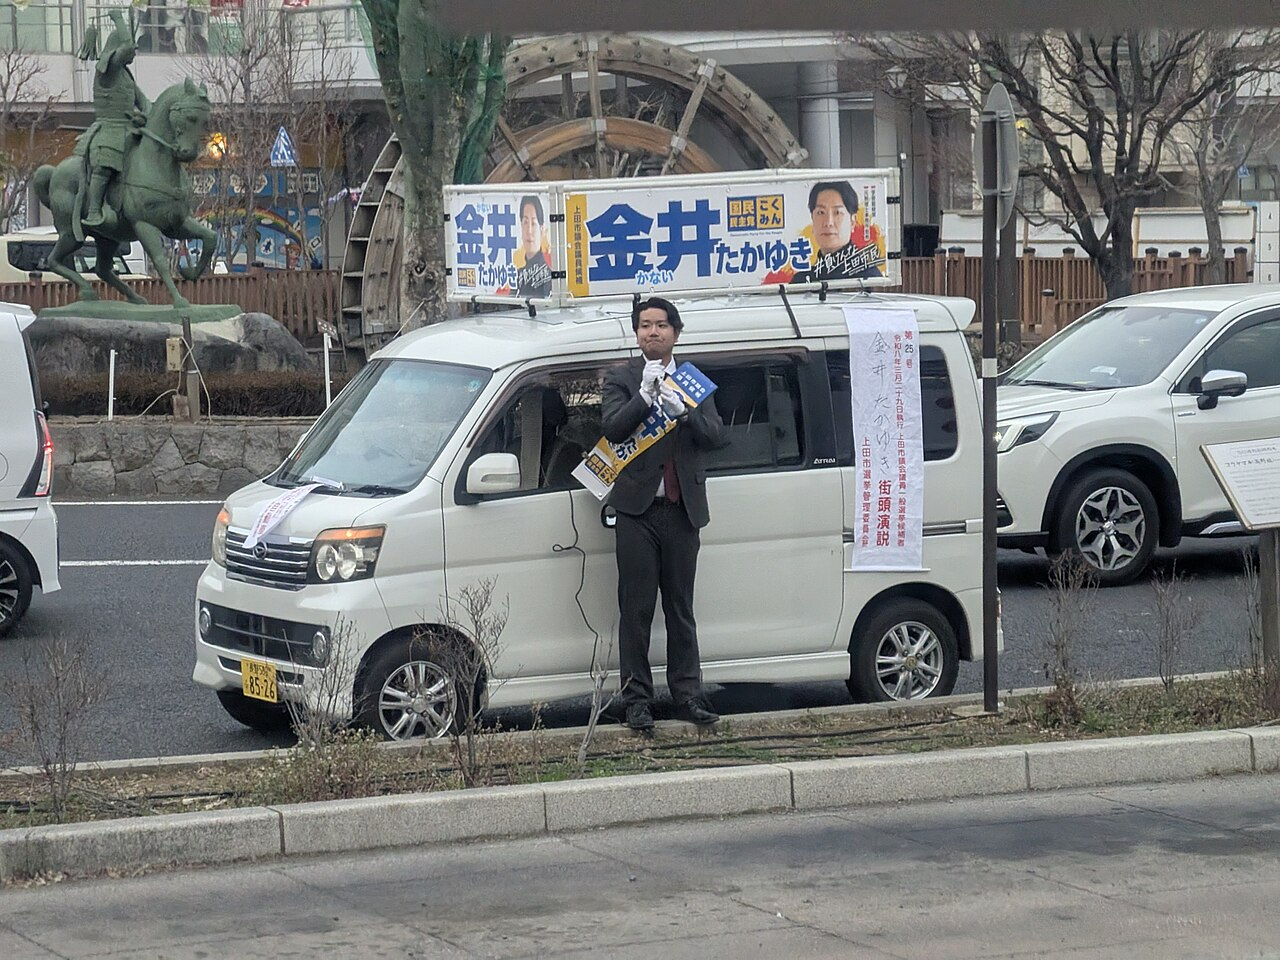
\includegraphics[width=0.48\linewidth,height=3.5cm,keepaspectratio]{Politician_in_front_of_Ueda_station.jpg}}\hfill
        \makebox[0.48\linewidth]{
\includegraphics[width=0.48\linewidth,height=3.5cm,keepaspectratio]{Politician_in_front_of_Ueda_station_masked.png}}
        \caption{Scena davanti alla stazione di Ueda. TruFor: $0{,}0156$; pixel non neri: $0{,}00\%$.}
        \label{fig:maschere-esempio-ueda}
    \end{subfigure}
    \par\medskip
    \begin{subfigure}{\linewidth}
        \centering
        \makebox[0.48\linewidth]{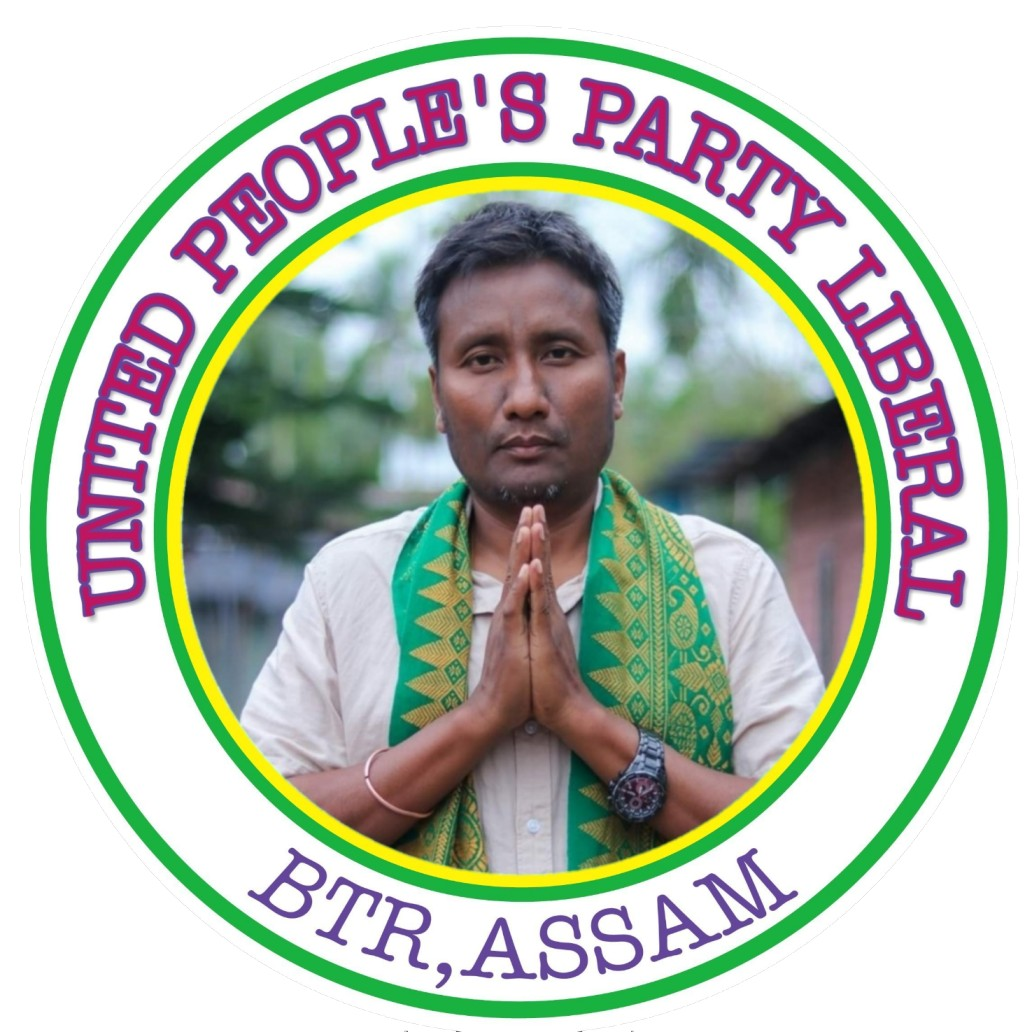
\includegraphics[width=0.48\linewidth,height=3.5cm,keepaspectratio]{Rakesh_Brahma,_EM_Bodoland_Territorial_Region.jpg}}\hfill
        \makebox[0.48\linewidth]{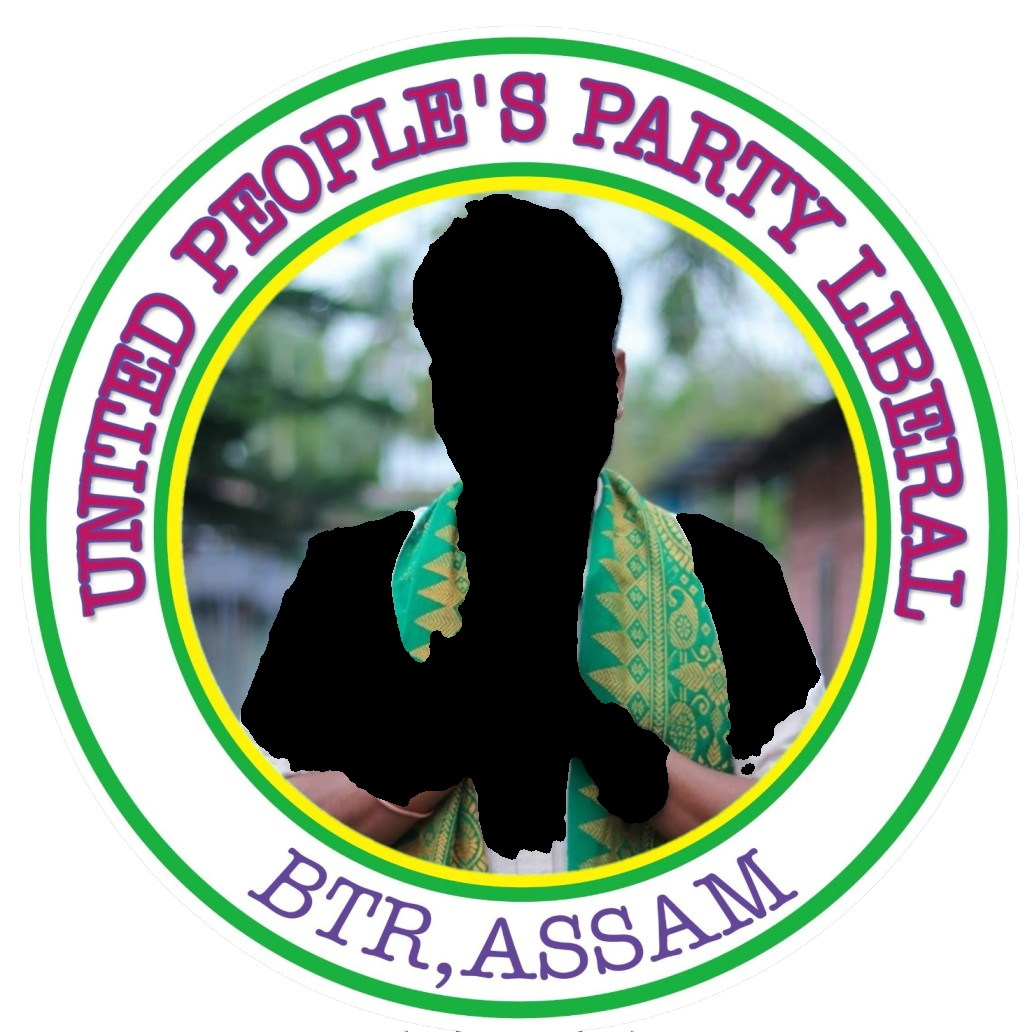
\includegraphics[width=0.48\linewidth,height=3.5cm,keepaspectratio]{Rakesh_Brahma,_EM_Bodoland_Territorial_Region_masked.png}}
        \caption{Ritratto con cornice grafica. TruFor: $0{,}9043$; pixel non neri: $85{,}09\%$.}
        \label{fig:maschere-esempio-brahma}
    \end{subfigure}
    \par\medskip
    \begin{subfigure}{\linewidth}
        \centering
        \makebox[0.48\linewidth]{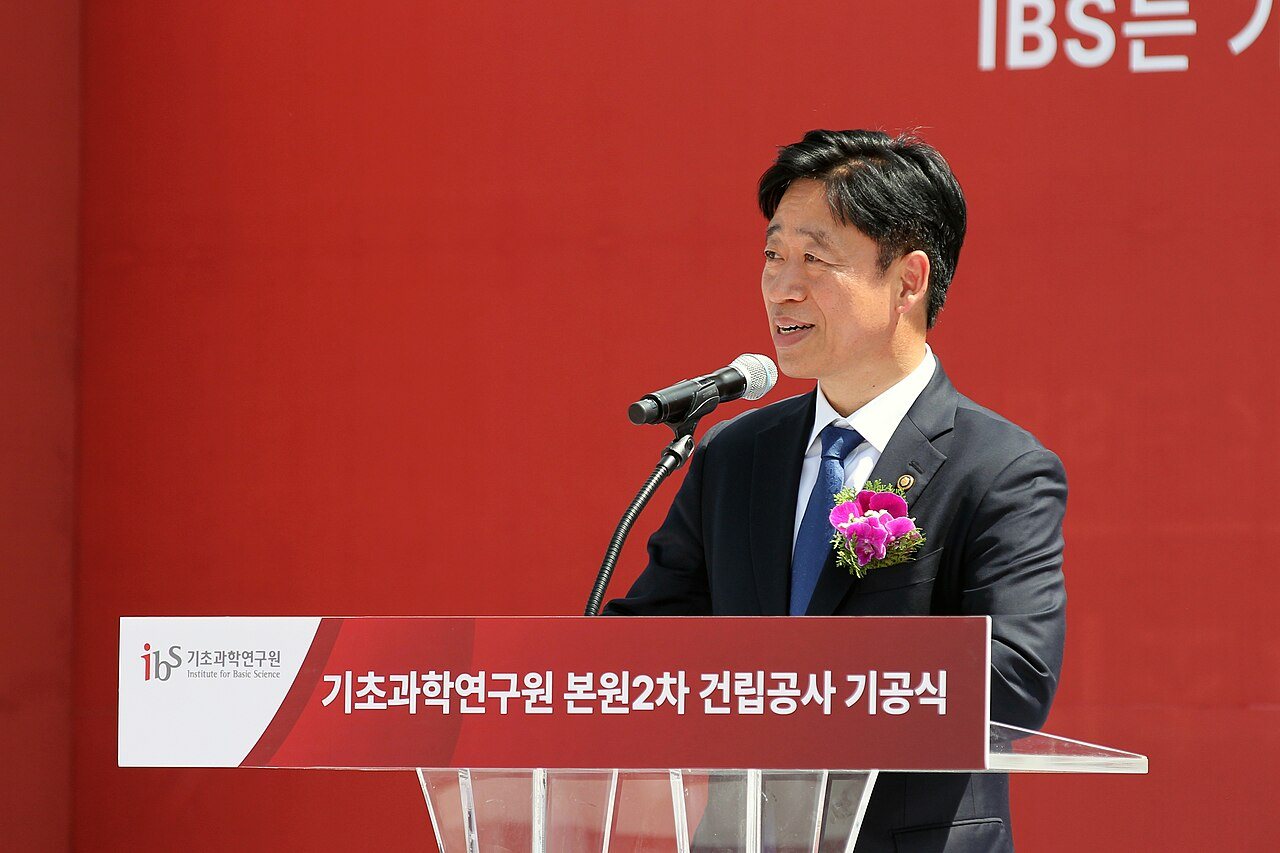
\includegraphics[width=0.48\linewidth,height=3.5cm,keepaspectratio]{South_Korean_politician_조승래.jpg}}\hfill
        \makebox[0.48\linewidth]{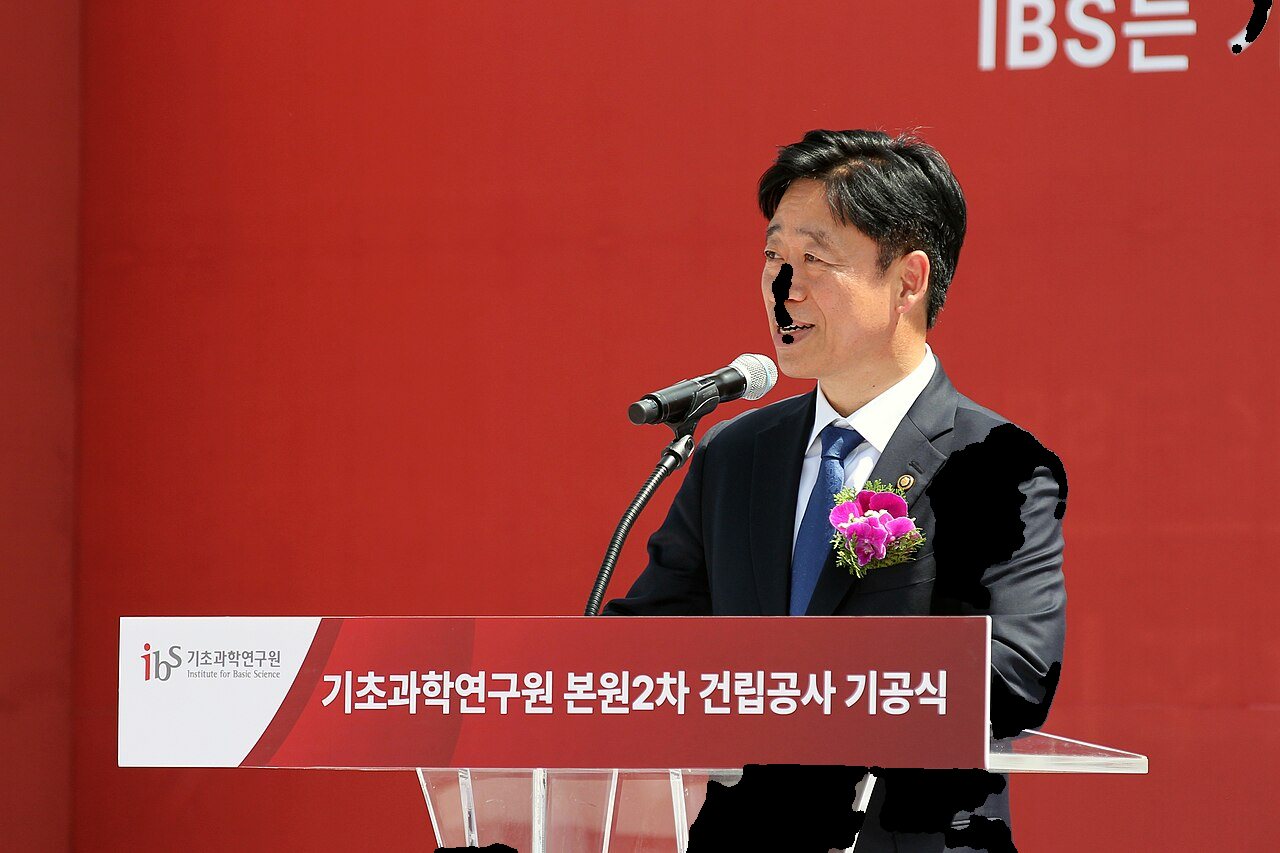
\includegraphics[width=0.48\linewidth,height=3.5cm,keepaspectratio]{South_Korean_politician_조승래_masked.png}}
        \caption{Discorso al podio. TruFor: $0{,}1124$; pixel non neri: $96{,}27\%$.}
        \label{fig:maschere-esempio-podio}
    \end{subfigure}
    \par\medskip
    \begin{subfigure}{\linewidth}
        \centering
        \makebox[0.48\linewidth]{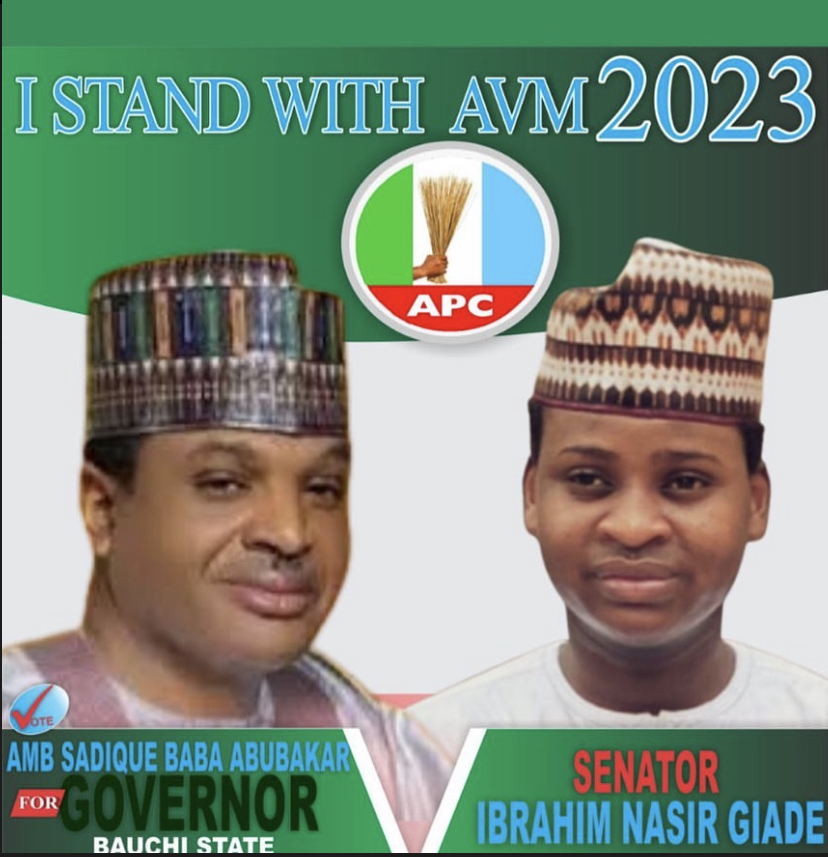
\includegraphics[width=0.48\linewidth,height=3.5cm,keepaspectratio]{Young_Politician_Naseer_Giade.jpg}}\hfill
        \makebox[0.48\linewidth]{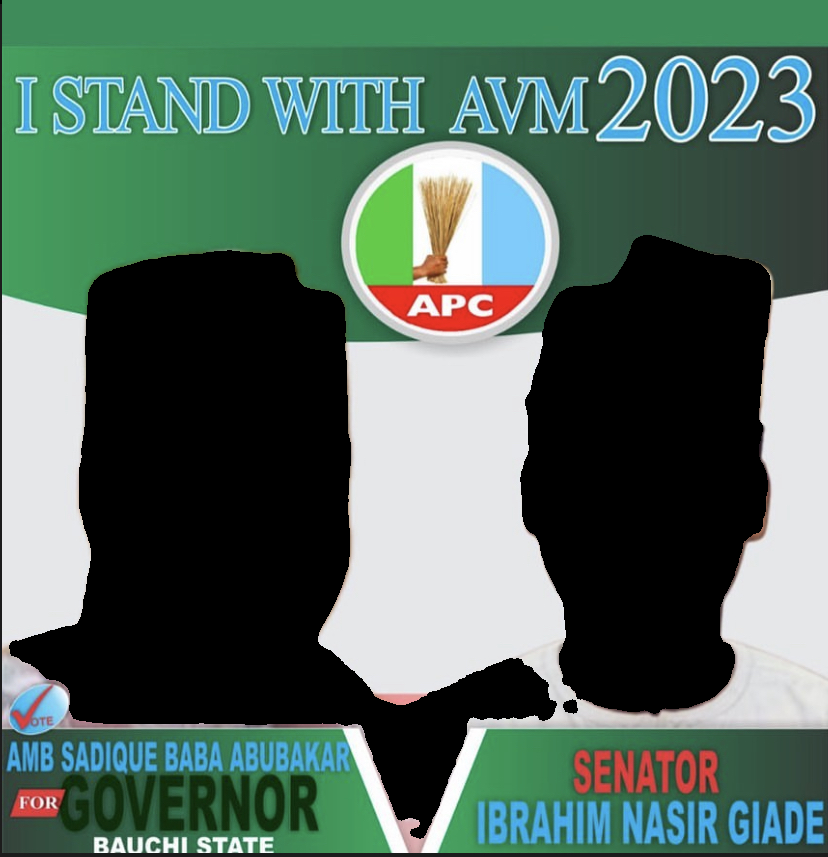
\includegraphics[width=0.48\linewidth,height=3.5cm,keepaspectratio]{Young_Politician_Naseer_Giade_masked.png}}
        \caption{Manifesto elettorale. TruFor: $0{,}9307$; pixel non neri: $67{,}43\%$.}
        \label{fig:maschere-esempio-manifesto}
    \end{subfigure}
    \caption[Mascheramento dei quattro esempi]{Mascheramento dei quattro esempi. I pixel neri indicano le regioni escluse. Fonti: \subref{fig:maschere-esempio-ueda}, \href{https://commons.wikimedia.org/wiki/File:Politician_in_front_of_Ueda_station.jpg}{Syced}; \subref{fig:maschere-esempio-brahma}, \href{https://commons.wikimedia.org/wiki/File:Rakesh_Brahma,_EM_Bodoland_Territorial_Region.jpg}{Swrang Borgoary}; \subref{fig:maschere-esempio-podio}, \href{https://commons.wikimedia.org/wiki/File:South_Korean_politician_조승래.jpg}{Rickinasia}; \subref{fig:maschere-esempio-manifesto}, \href{https://commons.wikimedia.org/wiki/File:Young_Politician_Naseer_Giade.jpg}{Naseer001}.}
    \label{fig:maschere-esempi}
\end{minipage}
\bigskip

\section{Descrizione testuale delle regioni sospette}
\label{sec:metodi-descrizioni}

Con \path{scripts/describe.py} trasformo le immagini mascherate nel campo \texttt{anomaly\_txt}, definito nella Sottosezione~\ref{subsec:materiali-descrizioni}. Uso BLIP per descrivere il contenuto visivo e EasyOCR per estrarre le scritte. La Figura~\ref{fig:descrizione-flusso} riassume il percorso degli input che superano il controllo sull'area visibile.

\begin{figure}[htbp]
    \centering
    \begin{tikzpicture}[
        box/.style={draw, rounded corners, align=center, font=\small, minimum height=1cm, text width=2.1cm},
        flow/.style={-{Latex}, thick}
    ]
        \node[box] (input) at (0,0) {Immagine\\mascherata};
        \node[box] (crop) at (2.9,0) {Ritaglio del\\contenuto visibile};
        \node[box] (blip) at (5.8,0.9) {BLIP\\Didascalia};
        \node[box] (ocr) at (5.8,-0.9) {EasyOCR\\Parole lette};
        \node[box, text width=2.7cm] (text) at (9,0) {Normalizzazione\\e unione};
        \draw[flow] (input) -- (crop);
        \draw[flow] (crop.east) -- (blip.west);
        \draw[flow] (crop.east) -- (ocr.west);
        \draw[flow] (blip.east) -- (text.west);
        \draw[flow] (ocr.east) -- (text.west);
    \end{tikzpicture}
    \caption{Costruzione della descrizione per le immagini con più del $2\%$ di pixel non neri. BLIP e OCR ricevono lo stesso ritaglio; normalizzo e unisco i rispettivi output nel campo \texttt{anomaly\_txt}.}
    \label{fig:descrizione-flusso}
\end{figure}

\subsection{Modelli e formato della descrizione}
\label{subsec:materiali-descrizioni}

Per descrivere le regioni sospette uso le immagini a colori su sfondo nero prodotte dal mascheramento automatico e salvate in \path{scripts/temp/masked/}.

Per BLIP~\cite{pmlr-v162-li22n}, descritto nella Sottosezione~\ref{subsec:background-blip}, adotto il modello \texttt{Salesforce/blip-image-captioning-large}, distribuito su \href{https://huggingface.co/Salesforce/blip-image-captioning-large}{Hugging Face}. Lo carico attraverso le classi \texttt{BlipProcessor} e \texttt{BlipForConditionalGeneration} della libreria Transformers~\cite{wolf-etal-2020-transformers}. Il processore prepara le immagini per la rete e converte i token generati in testo. Fornisco soltanto l'immagine, senza un testo iniziale che orienti la didascalia.

Per l'OCR uso EasyOCR~\cite{easyocr_software}, specificato nella Sottosezione~\ref{subsec:background-ocr}, con le lingue italiano e inglese. Con questa combinazione, il lettore predefinito carica il rilevatore CRAFT e il riconoscitore \texttt{latin\_g2}, basato sull'architettura CRNN. Mantengo i pesi distribuiti per entrambi gli strumenti, senza un ulteriore addestramento sul dataset politico.

Raccolgo il risultato nel campo \texttt{anomaly\_txt} di \path{dataset_filtered.csv}, associato a ciascuna immagine tramite \texttt{filename}. Il campo contiene la didascalia inglese normalizzata, seguita dalle parole riconosciute dall'OCR, oppure l'etichetta convenzionale \texttt{nomask}. Quest'ultima segnala l'assenza di una descrizione utilizzabile secondo il controllo dell'area visibile (Sottosezione~\ref{subsec:metodi-descrizioni-input}) e la normalizzazione del testo (Sottosezione~\ref{subsec:metodi-descrizioni-output}).

La rappresentazione può mescolare inglese e italiano e serve come input per la successiva analisi testuale.

\subsection{Controllo dell'area visibile e ritaglio}
\label{subsec:metodi-descrizioni-input}

Prima di interrogare i modelli misuro la frazione di pixel non neri nell'immagine mascherata. Se questa frazione non supera la soglia indicata nella Tabella~\ref{tab:descrizioni-parametri}, assegno \texttt{nomask} e salto sia BLIP sia l'OCR, per evitare la generazione di testo da input con contenuto visibile assente o limitato. Questa condizione può verificarsi anche per regioni selezionate piccole o contenenti pixel originariamente neri, indistinguibili dallo sfondo del mascheramento. L'etichetta \texttt{nomask} indica quindi l'esclusione dalla descrizione, non l'autenticità dell'immagine.

Per le altre immagini ritaglio il rettangolo che racchiude tutti i pixel non neri, aggiungendo un margine entro i bordi dell'immagine. Fornisco lo stesso ritaglio a BLIP ed EasyOCR, riducendo la cornice nera intorno al contenuto. Le aree nere interne rimangono tali e le eventuali regioni separate vengono descritte insieme.

\subsection{Generazione della didascalia e lettura delle scritte}
\label{subsec:metodi-descrizioni-modelli}

Elaboro le immagini in gruppi e carico i modelli una sola volta per esecuzione. Salto i file illeggibili. Riporto nella Tabella~\ref{tab:descrizioni-parametri} i parametri della configurazione corrente, definiti in \path{scripts/config.py}.

Uso BLIP in precisione a 32 bit, selezionando nell'ordine NVIDIA CUDA, Apple MPS o la CPU secondo la disponibilità. Per generare le didascalie uso la \emph{beam search}: a ogni passo seleziono più sequenze candidate e restituisco quella con il punteggio finale migliore.

Per controllare la lunghezza della didascalia generata da BLIP, imposto un numero minimo e massimo di nuovi token per immagine. Penalizzo il riuso dei token già presenti e impedisco la ripetizione di sequenze di lunghezza prefissata. Mantengo disattivato il campionamento casuale. I parametri di temperatura, selezione probabilistica e seme casuale previsti per la modalità alternativa restano quindi inattivi. Queste impostazioni agiscono durante la generazione, prima della normalizzazione del testo e dell'aggiunta delle parole riconosciute dall'OCR.

Configuro EasyOCR per eseguire i calcoli sulla GPU, quando disponibile, così da velocizzare il riconoscimento delle scritte. In assenza di una GPU compatibile, il programma usa la CPU. Richiedo un ingrandimento prima del rilevamento, per favorire la localizzazione delle scritte piccole. Conservo le trascrizioni che raggiungono la soglia di confidenza, le normalizzo come descritto nella Sottosezione~\ref{subsec:metodi-descrizioni-output} e scarto le parole che non raggiungono la lunghezza minima prevista. Ordino le parole candidate per confidenza decrescente del rispettivo riquadro, elimino i duplicati e ne limito il numero. L'ordine delle parole nell'immagine non è conservato. Questo limite riduce il peso delle immagini dense di testo. Se l'OCR fallisce su una singola immagine, mantengo la sola didascalia di BLIP.

Salvo le descrizioni di ogni gruppo completato in \path{description_temp.csv}. In caso di interruzione, riparto saltando i file già registrati. La ripresa presuppone che modelli, maschere e parametri restino gli stessi.

Al termine unisco le descrizioni a \path{dataset_filtered.csv} tramite \texttt{filename}, conservando solo le osservazioni corrispondenti e prive di valori mancanti. Rimuovo quindi il file intermedio.

\begin{table}[htbp]
    \centering
    \small
    \caption{Parametri per la descrizione delle immagini mascherate. La lunghezza BLIP è espressa in token; i limiti OCR riguardano le parole dopo la normalizzazione~\cite{pmlr-v162-li22n, easyocr_software}.}
    \label{tab:descrizioni-parametri}
    \begin{tabular}{@{}llr@{}}
        \toprule
        Componente & Parametro & Valore \\
        \midrule
        Input & Soglia di pixel non neri per \texttt{nomask} & $\leq 2\%$ \\
              & Ritaglio al rettangolo non nero & Attivo \\
              & Margine del ritaglio & 10 pixel \\
        \addlinespace
        BLIP & Sequenze candidate nella beam search & 5 \\
             & Nuovi token, minimo-massimo & 5--40 \\
             & Penalità di ripetizione & $1{,}3$ \\
             & Lunghezza delle sequenze non ripetibili & 2 token \\
             & Campionamento casuale & Disattivato \\
             & Rimozione delle parole duplicate & Attiva \\
        \addlinespace
        OCR & Lingue & Italiano, inglese \\
            & Fattore di ingrandimento richiesto & $1{,}5$ \\
            & Confidenza minima del riquadro & $0{,}65$ \\
            & Lunghezza minima delle parole & 3 lettere \\
            & Numero massimo di parole distinte & 20 \\
        \addlinespace
        Esecuzione & Immagini per gruppo & 30 \\
        \bottomrule
    \end{tabular}
\end{table}

\newpage
\subsection{Normalizzazione e unione del testo}
\label{subsec:metodi-descrizioni-output}

Applico la funzione \texttt{clean\_text} separatamente alla didascalia di BLIP e alle trascrizioni di EasyOCR. Riconduco le lettere accentate alla forma senza accento, converto il testo in minuscolo e sostituisco ogni carattere diverso da \texttt{a--z} con uno spazio. Nella didascalia mantengo solo la prima occorrenza di ciascuna parola; nell'OCR elimino i duplicati durante la selezione per confidenza. Concateno infine i due contributi. Una parola presente in entrambi può quindi comparire due volte nel risultato. Se la stringa finale è vuota, assegno \texttt{nomask}.

Queste scelte preparano il testo per un'analisi lessicale. Rimuovendo le cifre, perdo informazioni come anni e i numeri presenti nelle date; il limite minimo OCR esclude anche sigle di due lettere. Conservo in questa fase articoli e preposizioni. La rimozione delle parole funzionali, o \emph{stop word}, si effettua nella successiva vettorizzazione.

\subsection{Controllo delle descrizioni e limiti}
\label{subsec:metodi-descrizioni-controllo}

Produco \path{description_report.txt} con il numero di risultati, il conteggio di \texttt{nomask}, la lunghezza minima, mediana e massima e le dieci parole più frequenti. Riporto i valori nella Sottosezione~\ref{subsec:risultati-descrizioni}. Calcolo lunghezze e frequenze soltanto sulle descrizioni diverse da \texttt{nomask}, dopo l'unione di BLIP e OCR. Queste statistiche permettono di controllare la copertura e la distribuzione del testo prodotto. Per misurarne la correttezza servirebbero didascalie e trascrizioni di riferimento, distinte dalle annotazioni forensi.

La descrizione eredita i limiti della maschera: parti escluse possono interrompere parole o rimuovere il contesto necessario a interpretare un oggetto. BLIP può generare dettagli assenti, cioè \emph{allucinazioni}, oppure descrivere lo sfondo nero introdotto dalla procedura. Anche l'OCR può produrre letture errate dopo il filtraggio. Considero quindi \texttt{anomaly\_txt} una rappresentazione da valutare nelle analisi successive, anziché una verifica delle manipolazioni.

Mostro gli effetti del mascheramento nella Sottosezione~\ref{subsec:risultati-maschere-esempi} e le descrizioni ottenute nella Sottosezione~\ref{subsec:risultati-descrizioni-esempi}. Illustro la perdita di contesto, gli errori nel testo e l'interpretazione delle aree nere introdotte dalla maschera.

\subsection{Risultati delle descrizioni sul dataset}
\label{subsec:risultati-descrizioni}

Riporto nella Tabella~\ref{tab:risultati-descrizioni} i risultati del report \path{description_report.txt}, prodotto con la procedura della Sezione~\ref{sec:metodi-descrizioni}. Su 1.211 immagini ottengo 898 descrizioni testuali ($74{,}15\%$) e 313 etichette \texttt{nomask} ($25{,}85\%$).

\begin{table}[htbp]
    \centering
    \small
    \caption{Riepilogo delle descrizioni e dieci parole più frequenti, da \texttt{description\_report.txt}. Lunghezze e frequenze escludono \texttt{nomask}.}
    \label{tab:risultati-descrizioni}
    \begin{tabular}{@{}lr@{}}
        \toprule
        Misura & Valore \\
        \midrule
        Immagini con risultato archiviato & 1.211 \\
        Etichette \texttt{nomask} & 313 \\
        Lunghezza minima & 5 parole \\
        Lunghezza mediana & 17 parole \\
        Lunghezza massima & 36 parole \\
        \midrule
        Parola & Occorrenze \\
        \midrule
        \texttt{a} & 865 \\
        \texttt{is} & 727 \\
        \texttt{of} & 666 \\
        \texttt{there} & 659 \\
        \texttt{in} & 415 \\
        \texttt{man} & 401 \\
        \texttt{with} & 395 \\
        \texttt{and} & 309 \\
        \texttt{picture} & 246 \\
        \texttt{poster} & 199 \\
        \bottomrule
    \end{tabular}
\end{table}

La quota di \texttt{nomask} va interpretata secondo le condizioni definite nelle Sottosezioni~\ref{subsec:metodi-descrizioni-input} e~\ref{subsec:metodi-descrizioni-output}.

Le lunghezze contano le parole dopo la normalizzazione e l'unione di BLIP e OCR, quindi hanno un significato diverso dal limite di 5--40 token imposto alla generazione BLIP. Tra i termini più frequenti prevalgono parole funzionali inglesi e compaiono anche \texttt{man}, \texttt{picture} e \texttt{poster}.

Le descrizioni ottenute sono disponibili per la successiva analisi dell'engagement. Le statistiche ne descrivono la copertura e la composizione, ma non misurano la correttezza delle didascalie o delle trascrizioni. Il campo finale unisce i due contributi e non permette di valutarli separatamente.

\subsection{Descrizioni degli esempi visivi}
\label{subsec:risultati-descrizioni-esempi}

Nella Tabella~\ref{tab:descrizioni-esempi-commons} riporto il campo \texttt{anomaly\_txt} ottenuto dalle immagini mascherate della Sottosezione~\ref{subsec:risultati-maschere-esempi}. Questi quattro esempi rimangono separati dal riepilogo delle 1.211 immagini del dataset politico, descritto nella Tabella~\ref{tab:risultati-descrizioni}.

\begin{table}[htbp]
    \centering
    \small
    \caption{Descrizioni delle immagini mascherate mostrate nella Figura~\ref{fig:maschere-esempi}.}
    \label{tab:descrizioni-esempi-commons}
    \begin{tabular}{@{}>{\raggedright\arraybackslash}p{0.23\linewidth}>{\raggedright\arraybackslash}p{0.72\linewidth}@{}}
        \toprule
        Esempio & Testo finale \\
        \midrule
        \subref{fig:maschere-esempio-ueda}. Scena a Ueda & \texttt{nomask} \\
        \addlinespace
        \subref{fig:maschere-esempio-brahma}. Ritratto con cornice & \texttt{logo of united people s party library with silhouette a person party assan} \\
        \addlinespace
        \subref{fig:maschere-esempio-podio}. Discorso al podio & \texttt{there is a man standing at podium in front of microphone} \\
        \addlinespace
        \subref{fig:maschere-esempio-manifesto}. Manifesto elettorale & \texttt{there are two silhouettes of a man and woman facing each other for senator apc bauchi state ote amb sadique baba abubakar governor} \\
        \bottomrule
    \end{tabular}
\end{table}

Nell'esempio~\subref{fig:maschere-esempio-ueda} l'immagine mascherata è interamente nera: assegno quindi \texttt{nomask} senza interrogare BLIP e EasyOCR. Nell'esempio~\subref{fig:maschere-esempio-podio} la descrizione richiama l'uomo al podio e il microfono, ancora visibili dopo il mascheramento. Il testo finale non riporta le scritte coreane; il lettore OCR è configurato per italiano e inglese.

Gli esempi~\subref{fig:maschere-esempio-brahma} e~\subref{fig:maschere-esempio-manifesto} mostrano come il mascheramento influenzi l'interpretazione del contenuto. Il testo richiama sagome che corrispondono alle aree nere introdotte dalla procedura. Nell'esempio~\subref{fig:maschere-esempio-brahma} la descrizione riconduce l'immagine a un logo e richiama il nome del partito, ma contiene anche termini errati: compaiono \texttt{library} e \texttt{assan} al posto delle scritte \texttt{LIBERAL} e \texttt{ASSAM}. Nell'esempio~\subref{fig:maschere-esempio-manifesto} descrive le aree nere come le sagome di un uomo e di una donna rivolti l'uno verso l'altra: attribuisce quindi caratteristiche che l'input mascherato non permette di ricavare. Il testo conserva informazioni presenti nelle scritte, tra cui \texttt{senator}, \texttt{apc}, \texttt{bauchi state} e \texttt{governor}. I due esempi mostrano così la presenza, nella stessa descrizione, di elementi riconoscibili, parole errate e interpretazioni delle forme prodotte dal mascheramento.

Questi risultati illustrano come il testo possa combinare contenuto utile, errori e riferimenti alle aree nere introdotte dalla procedura. Poiché il CSV contiene soltanto la stringa finale, non attribuisco i singoli termini a BLIP o a EasyOCR.
